\chapter{Learning Prob. Submodular Models} \label{ch:genes}

\section{Introduction}

\section{Sampling for Approximate Maximum Likelihood Learning}

\section{Application: Modeling Mutually Exclusive Cancer Genes}
\subsection{Previous Approaches}
\subsection{Experiments: Sythetic Data}
\subsection{Experiments: Real Cancer Data}

\begin{figure}[htb]
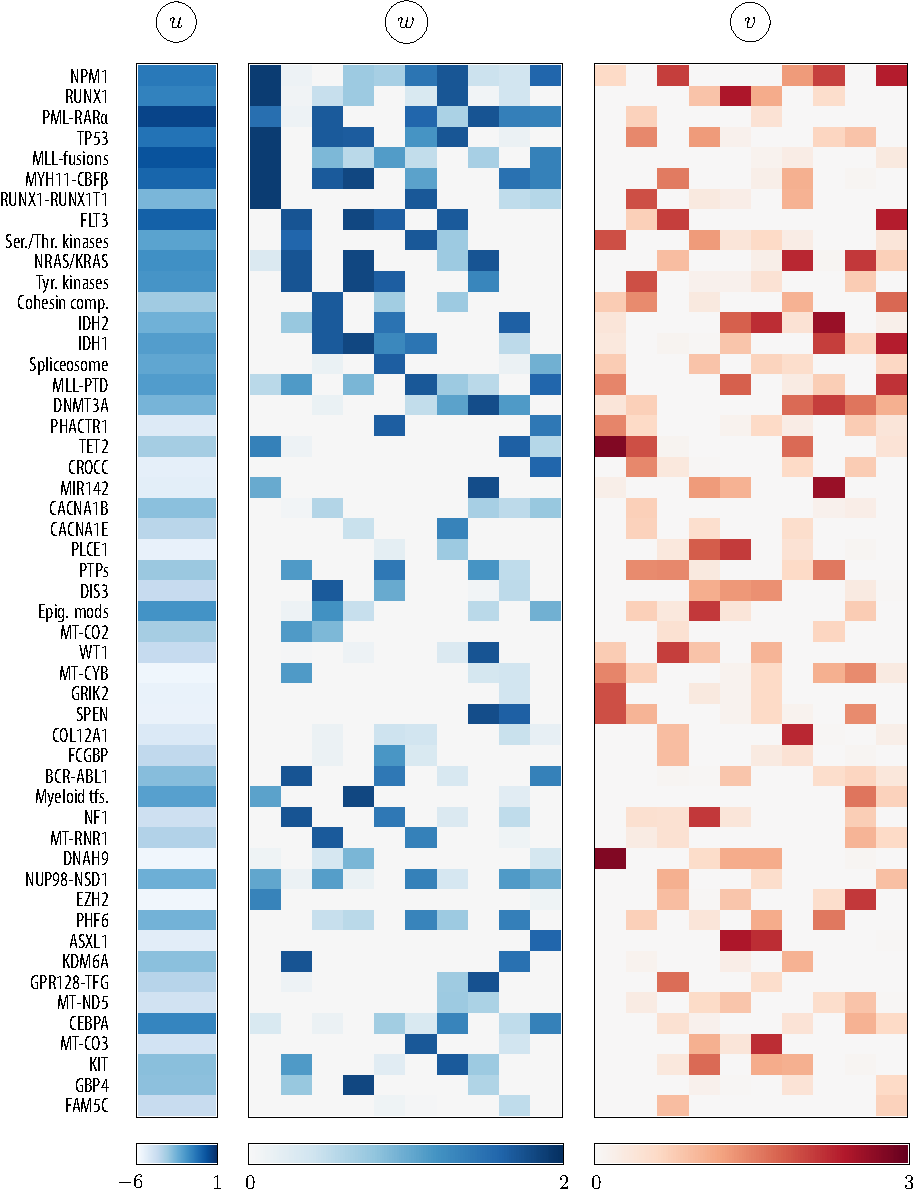
\includegraphics[width=\textwidth]{figures/genes/mat_aml.pdf}\\[2em]
\caption{Test}
\end{figure}

\begin{figure}[htb]
\centering
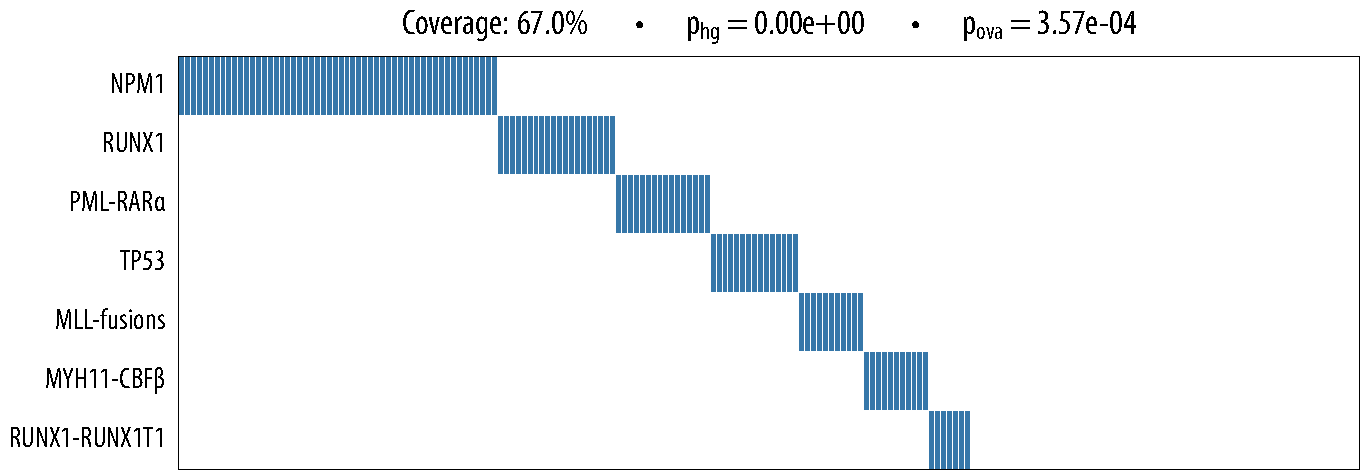
\includegraphics[width=\textwidth]{figures/genes/aml_1.pdf}\\[2em]
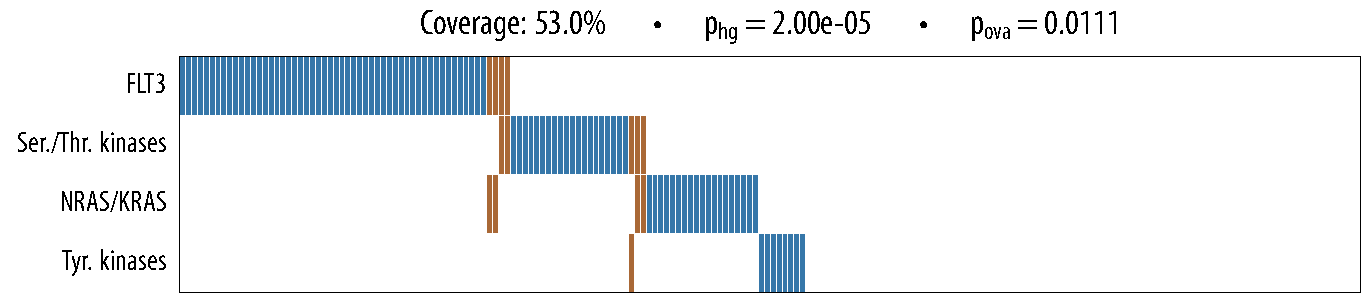
\includegraphics[width=\textwidth]{figures/genes/aml_2.pdf}\\[2em]
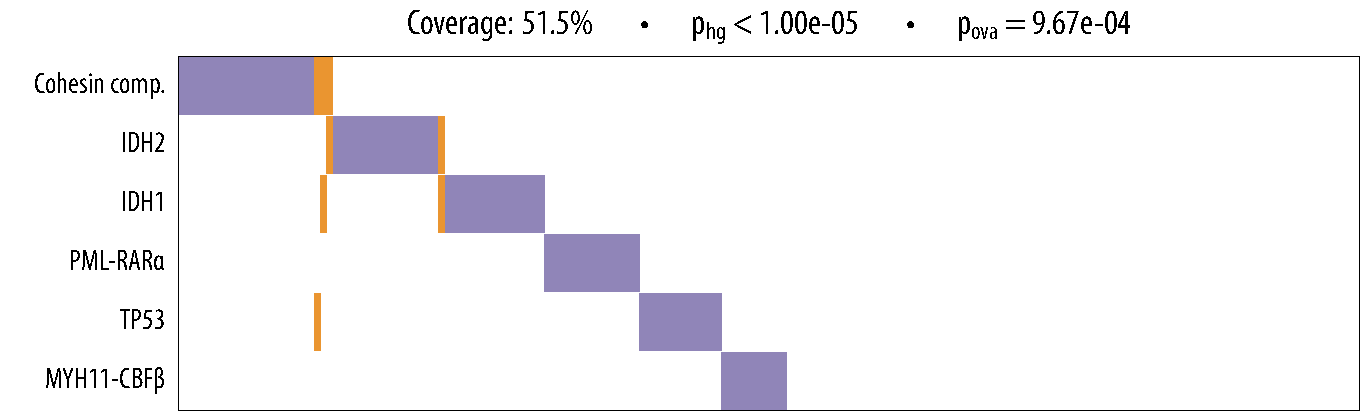
\includegraphics[width=\textwidth]{figures/genes/aml_3.pdf}\\[2em]
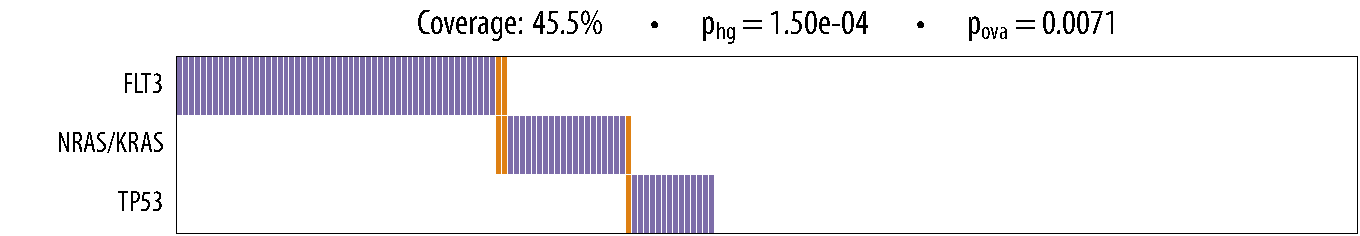
\includegraphics[width=\textwidth]{figures/genes/aml_4.pdf}\\[2em]
\caption{Test}
\end{figure}

\begin{figure}[htb]
\centering
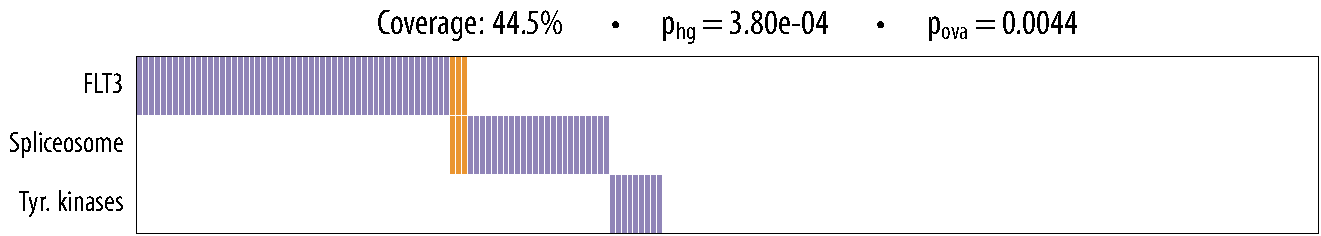
\includegraphics[width=\textwidth]{figures/genes/aml_5.pdf}\\[2em]
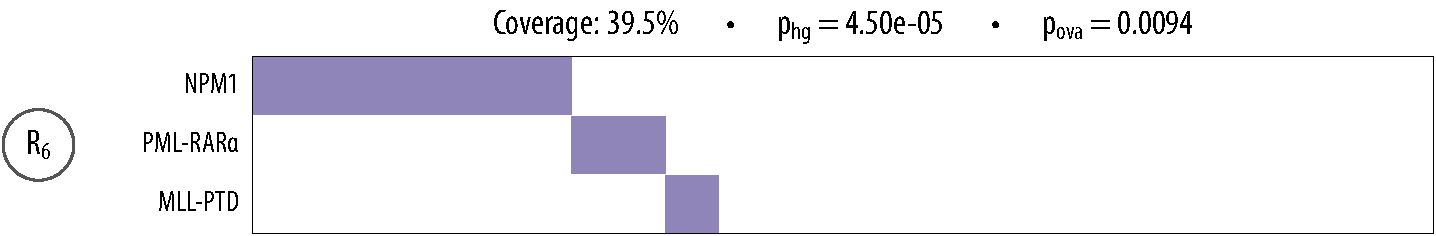
\includegraphics[width=\textwidth]{figures/genes/aml_6.pdf}\\[2em]
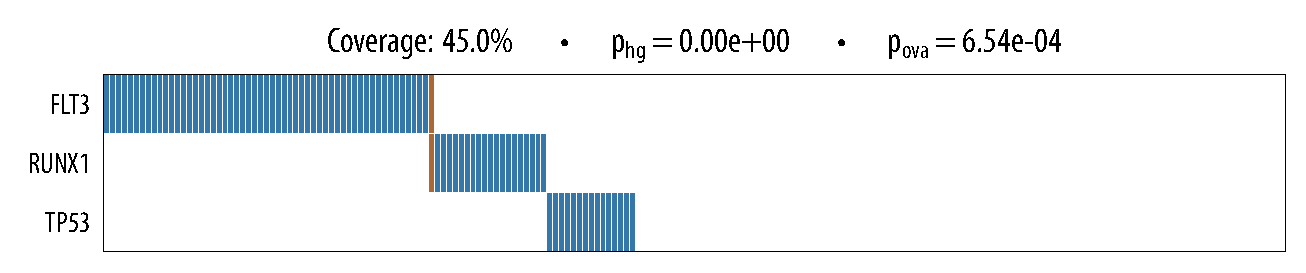
\includegraphics[width=\textwidth]{figures/genes/aml_7.pdf}\\[2em]
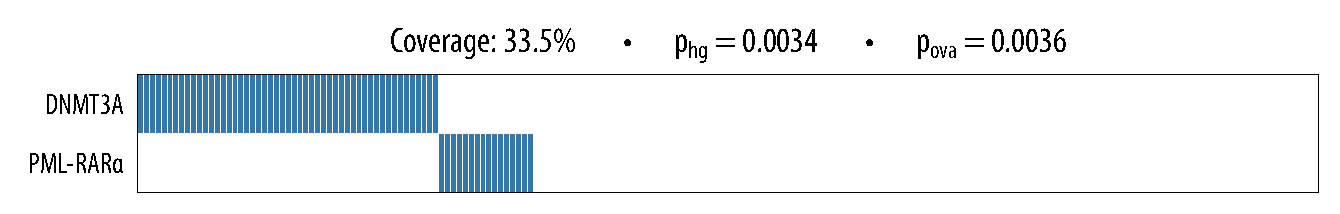
\includegraphics[width=\textwidth]{figures/genes/aml_8.pdf}\\[2em]
\caption{Test}
\end{figure}

\begin{figure}[htb]
\centering
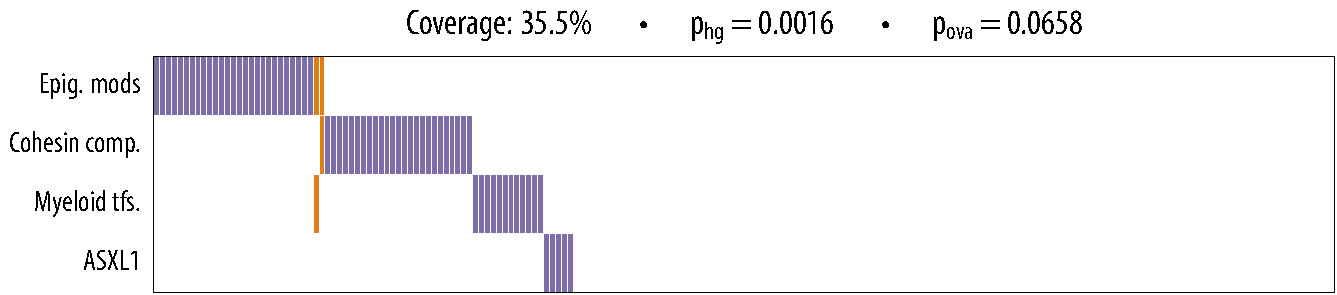
\includegraphics[width=\textwidth]{figures/genes/aml_comet1.pdf}\\[2em]
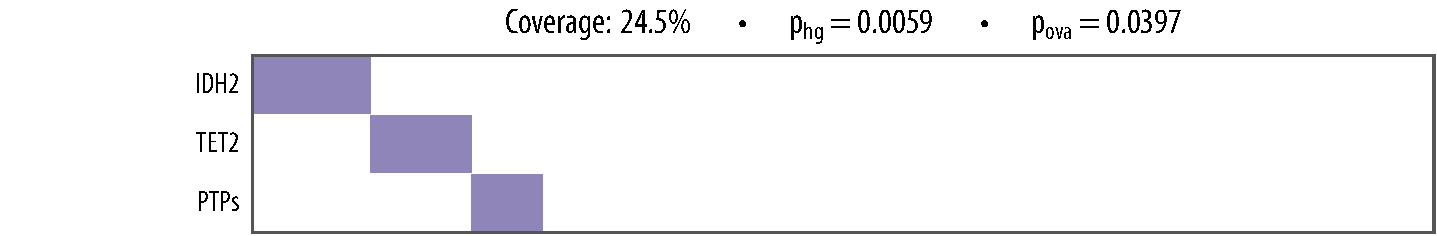
\includegraphics[width=\textwidth]{figures/genes/aml_comet2.pdf}\\[2em]
\caption{Test}
\end{figure}

\begin{figure}[htb]
\centering
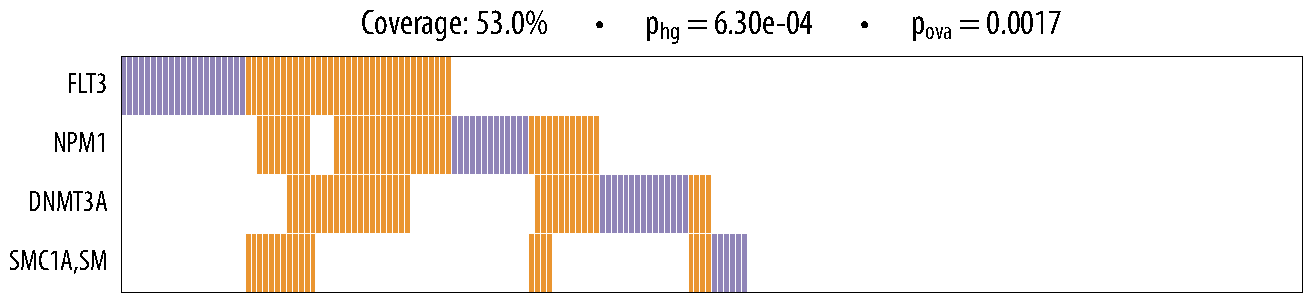
\includegraphics[width=\textwidth]{figures/genes/aml_1_a.pdf}\\[2em]
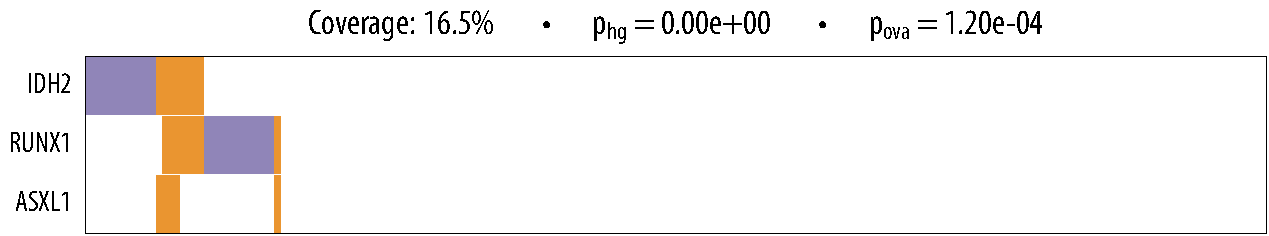
\includegraphics[width=\textwidth]{figures/genes/aml_3_a.pdf}\\[2em]
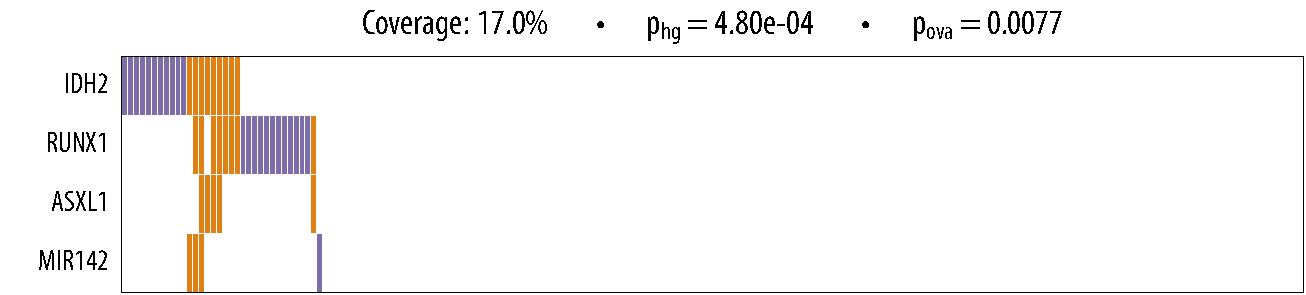
\includegraphics[width=\textwidth]{figures/genes/aml_2_a.pdf}\\[2em]
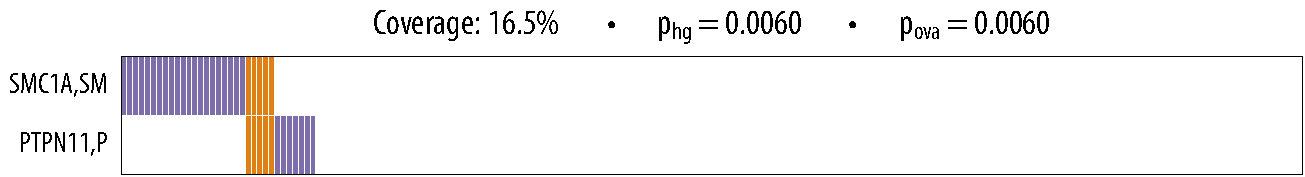
\includegraphics[width=\textwidth]{figures/genes/aml_6_a.pdf}\\[2em]
\caption{Test}
\end{figure}

\section{Conclusion}